\documentclass[12pt,a4paper]{article}

\usepackage[utf8]{inputenc}
\usepackage[english]{babel}
\usepackage{hyperref}
\usepackage{amssymb}
\usepackage{amsmath}
\usepackage{graphicx}
\usepackage{setspace}
\usepackage{float}
\usepackage[justification=centering]{caption}
\usepackage{tikz}
\usepackage{parskip}
\usetikzlibrary{positioning, calc, backgrounds, shapes.geometric}

\begin{document}

\begin{titlepage}
    \centering 
    \vspace{2.5cm} 
    {\Large \textbf{Reinforcement Learning on Gym's MiniGrid Interface}}\\[0.1cm]
    \vspace{1cm}
    \vspace{2cm}
    Georgios Lazaridis\\[0.5cm]
    AEM: 4419\\[1cm]
    
\includegraphics[width=0.3\textwidth]{images/auth.png}\\[0.5cm]
    \vspace{0.5cm}
    {\Large Aristotle University of Thessaloniki}
    \vfill
    {\Large May 2026}
    \vspace*{1cm} 
\end{titlepage}

\author{Georgios Lazaridis}

\pagenumbering{arabic} 
\centering
\section{Introduction and Implementation}
This project explores the application of Deep Reinforcement Learning using the \textbf{Proximal Policy Optimization (PPO)} algorithm within the \textit{Gym MiniGrid} framework. The core objective was to develop an agent capable of navigating complex, logic-driven environments through custom reward engineering and optimized neural architectures.

\subsection{Task Definition and Environment Components}
\begin{itemize}
    \item \textbf{Navigation Logic:} The agent must solve multi-stage puzzles requiring inventory management (key collection) and environment manipulation (unlocking doors). Three custom map classes (\texttt{First}, \texttt{Second}, and \texttt{Third}) were developed for this purpose.
    
    \item \textbf{Custom Entities:} To enhance environmental complexity, the \newline \texttt{RimWorldEnemy} class was implemented.
    
    \item \textbf{Observation Space:} Observations consist of a partially observable $11\times11$ grid. This spatial data is processed as an image-like tensor, allowing the agent to perceive both static terrain and dynamic threats.
\end{itemize}

\subsection{Architectural Refinements and Evaluation}
\begin{itemize}
    \item \textbf{Feature Extraction:} A custom \textbf{Convolutional Neural Network (CNN)} serves as the feature extractor.

    \item \textbf{Learning Dynamics:} The \textbf{PPO} algorithm was selected for its robust clipping mechanism, which prevents catastrophic policy updates during the critical phases of reward discovery.
    
    \item \textbf{Visual Evolution Monitoring:} To assess the agent's progress, \newline \texttt{video\_overlay.py} utility was developed. This script utilizes \textbf{OpenCV} to produce blended video comparisons (\texttt{.mp4}) between a baseline random agent and the trained PPO agents.
\end{itemize}

\section{Environment Layouts and Map Design}
To evaluate the agent's performance across different levels of complexity, three distinct environment classes were developed. Each map introduces unique spatial constraints and logic requirements.

\subsection{Map 1: Hazard Avoidance}
\begin{figure}[H]
    \centering
    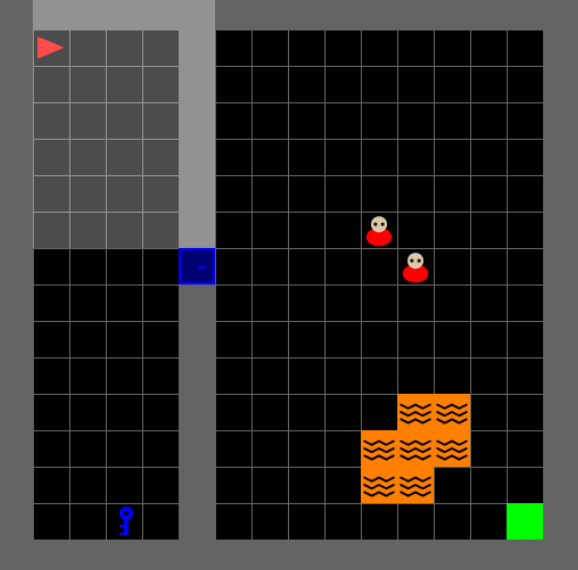
\includegraphics[width=0.45\textwidth]{images/first.png}
    \caption{\textbf{First Map:} A dual-room configuration featuring a locked door mechanism, lava hazards, and dynamic enemies.}
    \label{fig:map1}
\end{figure}
The \textit{First} map (see Figure \ref{fig:map1}) consists of a two-room layout separated by a locked door. The agent must navigate a simple corridor, avoid lava pits and Enemy entities to reach the goal (indicated by the green square).

\subsection{Map 2: Sequential Logic and Inventory Management}
\begin{figure}[H]
    \centering
    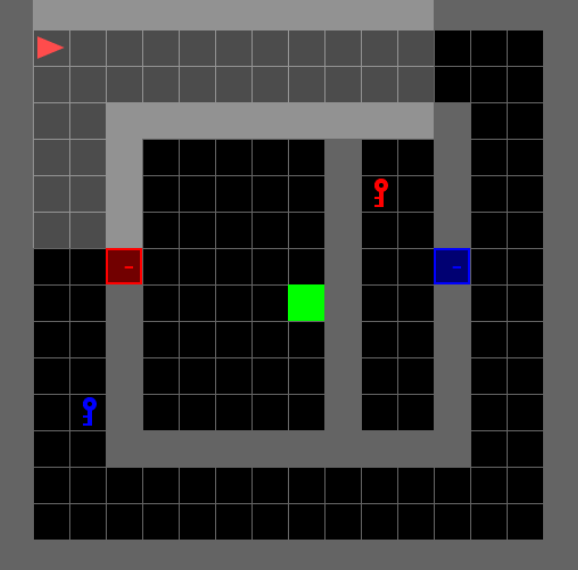
\includegraphics[width=0.45\textwidth]{images/second.png}
    \caption{\textbf{Second Map:} A multi-stage logic environment requiring key exchange and non-linear pathfinding.}
    \label{fig:map2}
\end{figure}
The \textit{Second} map (Figure \ref{fig:map2}) introduces a different design. It requires multi-stage logic where the agent must pick up a blue key, open the corresponding door, and subsequently drop the first key in order to handle a second key/door sequence before finding the goal.

\subsection{Map 3: Exploration and Spatial Generalization}
\begin{figure}[H]
    \centering
    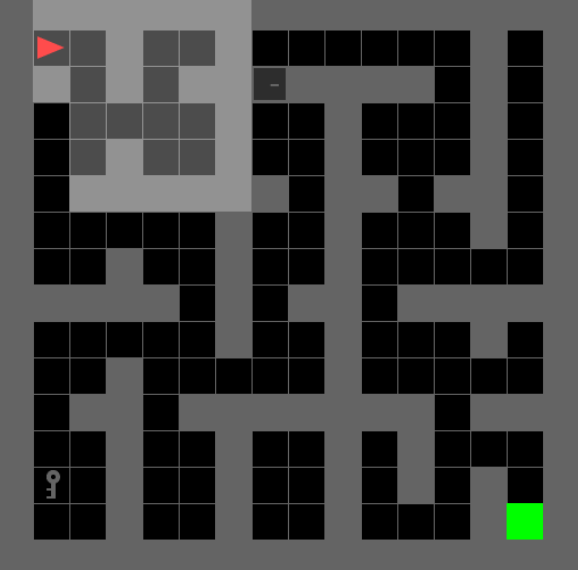
\includegraphics[width=0.45\textwidth]{images/third.png}
    \caption{\textbf{Third Map:} A dense navigation Maze focused on finding the Shortest Path.}
    \label{fig:map3}
\end{figure}
The final \textit{Third} environment (Figure \ref{fig:map3}) is a dense maze focused on pure navigation efficiency. The maze consists of several dead ends but lacks the enemies and inventory management the other two maps required.

\subsection{Custom Entity Rendering}
An extension to the environment's visual capabilities is the implementation of the \texttt{RimWorldEnemy} class. The render of the enemy was inspired by the style of games like \textit{RimWorld} and \textit{Prison Architect} to add some flavor.

\begin{figure}[H]
    \centering
    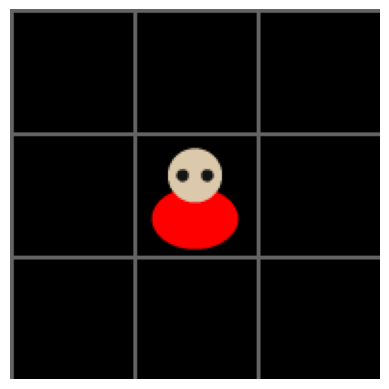
\includegraphics[width=0.2\textwidth]{images/enemy_render.png} 
    \caption{\textbf{Custom Enemy Sprite}}
    \label{fig:enemy}
\end{figure}

The rendering process (see \texttt{enemy.py}) utilizes \textbf{fill\_coords} to layer the body, clothing, and facial features in a specific Z-order, and a helper utility (\textbf{point\_in\_ellipse.py}) to define the boundaries for the color filling.

Similarly to the \texttt{Lava} object in \textit{MiniGrid}, any overlap with the \texttt{RimWorldEnemy} class triggers an immediate episode termination and a significant reward penalty. 

This addition introduces a higher level of visual and logical complexity; the \textbf{CNN} model is forced to distinguish between different "lethal" entities (e.g., orange static lava vs. red dynamic enemies), preventing the agent from relying on simple color-blob heuristics.

\section{Reward Engineering and Experimental Results}

\subsection{Dense Reward Shaping (Phase-Based Learning)}
To accelerate convergence, the global task was decomposed into a \textbf{Finite State Machine} with sub-goals:
\begin{itemize}
    \item \textbf{Navigation Guidance:} Implemented a "Compass" system using \textit{Manhattan Distance} to provide immediate mathematical feedback during the initial training phases.
    \item \textbf{Sub-goal Rewards:} Assigned discrete bonuses for critical actions (map-specific):
        \begin{itemize}
            \item \textbf{First map:} $+0.5$ for key pickup, $+1.0$ for opening the locked door; small per-step shaping for moving closer to the current phase target ($+0.1$ when distance decreases in Phases 1--2, and $+0.05$ when approaching the goal in Phase 3).
            \item \textbf{Second map:} Two sequential key/door phases with identical per-phase bonuses ($+0.5$ on key pickup, $+1.0$ on door open) and small front-cell shaping rewards when approaching the correct key/door.
            \item \textbf{Third map:} Exploration and visitation bonuses ($+0.005$ for new tiles).
        \end{itemize}
    \item \textbf{Time Penalty:} A constant step penalty of $-0.005$ is applied to incentivize shorter solutions.
    \item \textbf{Failure Penalties:} Collisions with lethal tiles or enemies, or catastrophic drop of inventory incur on larger negative rewards (map-dependent) and typically terminate the episode.
\end{itemize}

\section{Results and Evolution}
The codebase utilizes \textit{TensorBoard} logging for real-time monitoring of \texttt{ep\_rew\_mean} and \texttt{ep\_len\_mean}. TensorBoard runs for the trainings are under \texttt{app/data/runs/}.

\subsection{First Map}
\subsection{Second Map}
\subsection{Third Map}


\section{Code Implementation and Repository}
\begin{itemize}
    \item \textbf{Efficency:} The codebase utilizes \textbf{load} and \textbf{save} logic for agents for repeated deployment and testing between agents through the \texttt{video\_overlay.py} script
    \item \textbf{Saved Models:} Trained agents are saved at \texttt{app/data/model/}.
\end{itemize}

\section{GitHub Repository}
The complete source code and necessary configuration files for reproducing the experiments are publicly available on the GitHub repository:
\begin{itemize}
    \item \hyperlink{https://github.com/lazoulios/gym-minigrid}{https://github.com/lazoulios/gym-minigrid}
    \item \textbf{Contents:} This repository includes the main \textbf{train.py} script, custom map scripts \textbf{first\_map.py}, \textbf{second\_map.py} and \textbf{third\_map.py} the \textbf{enemy.py}, \textbf{point\_in\_ellipse.py} and \textbf{video\_overlay.py} files, the \textbf{requirements.txt} dependency list, and finally \textbf{README.md} setup instructions and overall structure report.
\end{itemize}

\end{document}